\begin{titlepage}

\begin{flushleft}
	
\includegraphics[height=1.5cm]{figs/LKR_Logo.png}
	\hfill
	%\includegraphics[height=1.5cm]{figs/MZH_Logo.png}
	%\hfill
	
\includegraphics[height=1.5cm]{figs/LUH_Logo.jpg}
\end{flushleft}

\vspace{10mm} 
\begin{center}
\Large{Vorlesung/Experimentelle \"Ubung: 

Programmierung mechatronischer Systeme

\vspace{5mm}

\textbf{Hausarbeit}}

\vspace{5mm}
\textbf{\LARGE{Raspberry Pi Roboter ("French Bulldog")}}
\end{center}

\vfill
% hier könnt ihr ein Bild eurer Roboters einfügen
\begin{center}
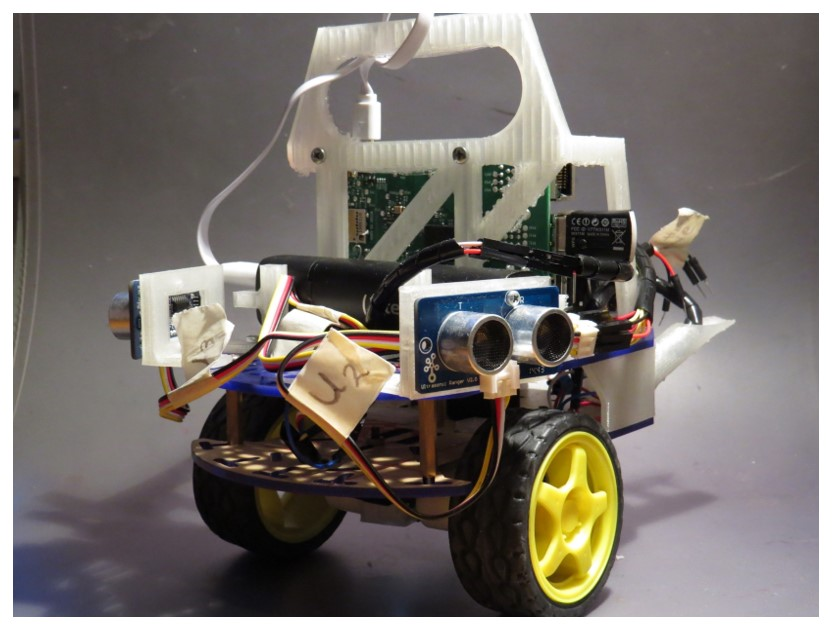
\includegraphics[width = 80mm]{figs/PiRobot.jpg}
\end{center}

\vfill

\begin{center}
\begin{tabular}{c c}
\large{Tobias Gieseking} & \large{Nils Melchert}\\
\large{Matrikelnummer 2883510} & \large{Matrikelnummer 2869520}
\end{tabular}
\end{center}
\vspace{15mm}

\begin{tabular}{l}
\large{Sommersemester 2016}\\
\large{Hannover, 15.07.2016}
\end{tabular}


\vspace{15mm}
{\large
\begin{tabular}{l l}
Dozentin:  & Prof. Dr.-Ing. Jessica Burgner\\
Betreuer: & M.Sc. Ernar Amanov und M.Sc. Carolin Fellmann\\
\end{tabular}
}

\end{titlepage}
